
\documentclass[10pt,english, openany]{book}
\usepackage[]{graphicx}
\usepackage[]{color}
\usepackage{algorithm}
\usepackage{algpseudocode}
\usepackage{amsmath}
\renewcommand{\algorithmicrequire}{\textbf{Input:}} 
\renewcommand{\algorithmicensure}{\textbf{Output:}}
\usepackage{listings}
\usepackage{alltt}
% \usepackage[T1]{fontenc}
% \usepackage[utf8]{inputenc}
\setcounter{secnumdepth}{3}
\setcounter{tocdepth}{3}
\setlength{\parskip}{\smallskipamount}
\setlength{\parindent}{0pt}

% Set page margins
\usepackage[top=100pt,bottom=100pt,left=100pt,right=100pt]{geometry}

% Package used for placeholder text
\usepackage{lipsum}

% Prevents LaTeX from filling out a page to the bottom
\raggedbottom

% Adding both languages
\usepackage[english]{babel}

% All page numbers positioned at the bottom of the page
\usepackage{fancyhdr}
\fancyhf{} % clear all header and footers
\fancyfoot[C]{\thepage}
\renewcommand{\headrulewidth}{0pt} % remove the header rule
\pagestyle{fancy}

% Changes the style of chapter headings
\usepackage{titlesec}
\titleformat{\chapter}
   {\normalfont\LARGE\bfseries}{\thechapter.}{1em}{}
% Change distance between chapter header and text
\titlespacing{\chapter}{0pt}{50pt}{2\baselineskip}

% Adds table captions above the table per default
\usepackage{float}
\floatstyle{plaintop}
\restylefloat{table}

% Adds space between caption and table
\usepackage[tableposition=top]{caption}

% Adds hyperlinks to references and ToC
\usepackage{hyperref}
\hypersetup{hidelinks,linkcolor = black} % Changes the link color to black and hides the hideous red border that usually is created

% If multiple images are to be added, a folder (path) with all the images can be added here 
\graphicspath{ {Figures/} }

% Separates the first part of the report/thesis in Roman numerals
\frontmatter

\lstset{
 % backgroundcolor=\color{lightgray}, 
 basicstyle = \footnotesize,       
 breakatwhitespace = false,        
 breaklines = true,                 
 captionpos = b,
 columns=fixed,                    
 commentstyle = \ttfamily,
 extendedchars = false,             
 frame=lrtb, 
 % framerule=0.5pt,
 keepspaces=true,
 keywordstyle=\bfseries, % keyword style
 language = C++,          
 otherkeywords={string}, 
 numbers=left, 
 numbersep=5pt,
 xleftmargin=5em,
 xrightmargin=10em,
 % numberstyle=\tiny\color{mygray},
 rulecolor=\color{black},         
 showspaces=false,  
 showstringspaces=false, 
 showtabs=false,    
 stepnumber=1,         
 stringstyle=\color{mymauve}, % string literal style
 tabsize=2,          
 % title=\lstname                      
}


%%%%%%%%%%%%%%%%%%%%%%%%%%%%%% Starts the document
\begin{document}

%%% Selects the language to be used for the first couple of pages
\selectlanguage{english}

%%%%% Adds the title page
\begin{titlepage}
	\clearpage\thispagestyle{empty}
	\centering
	\vspace{1cm}

	% Titles
	% Information about the University
	{\normalsize School of Computer Science and Technology \\ 
	Zhejiang University \par}
	\vspace{1cm}
	
	\begin{figure}[h]
		\centering
		
\includegraphics{Figures/ZJDX}
	\end{figure}	
	\vspace{1cm}
		
	{\Huge \textbf{Skip List}} \\
	%\vspace{1cm}
	%{\large \textbf{xxxxx} \par}
	\vspace{3cm}
	{\normalsize FIRST LAST \\ % \\ specifies a new line
	             FIRST LAST \\
	             FIRST LAST\par}
	\vspace{2cm}
    \begin{figure}[h]
    	\centering 
    	
\includegraphics{Figures/QSY}
    \end{figure}
       
    \vspace{0.5cm}
		
	% Set the date
	{\normalsize 2020-05-20 \par}
	
	\pagebreak

\end{titlepage}

% Adds a table of contents
\tableofcontents{}

%%%%%%%%%%%%%%%%%%%%%%%%%%%%%%%%%%%%%%%%%%%%%%%%%%%%%%%%%%%%%%%%%%%%%%%%%%%%%%%%%%%%%%%%%%%%
%%%%%%%%%%%%%%%%%%%%%%%%%%%%%%%%%%%%%%%%%%%%%%%%%%%%%%%%%%%%%%%%%%%%%%%%%%%%%%%%%%%%%%%%%%%%
%%%%% Text body starts here!
\mainmatter

\chapter{Introduction}
\textit{Skip list} is a data structure that allows $\mathcal O(\log n)$ search complexity as well as $\mathcal O(\log n)$ insertion complexity within an ordered sequence of $n$ elements. Thus it can get the best features of an array while maintaining a linked list-like structure that allows insertion, which is not possible in an array. 

Fast search is made possible by maintaining a linked hierarchy of subsequences, with each successive subsequence skipping over fewer elements than the previous one. 

Searching starts in the sparsest subsequence until two consecutive elements have been found, one smaller and one larger than or equal to the element searched for. Via the linked hierarchy, these two elements link to elements of the next sparsest subsequence, where searching is continued until finally we are searching in the full sequence.
\vspace{2cm}
\begin{figure}[h]
	\centering
	\includegraphics[scale = 0.4]{Figures/Linked_Lists}
	\caption{Linked Lists with Additional Pointers}
\end{figure}
\chapter{Algorithm Specification}
\section{Data Structures}
\subsection{Node}
To implement a skiplist, we should first define a Node class, this class contains the following elements:
\begin{enumerate}
	\item key: the key of a node
	\item value: the data of the node
	\item level: A level i node carries i forward pointers indexed through 0 to i.
	\item forward: store all pointers
\end{enumerate}

\begin{lstlisting}
class Node
{
private:
    
    int key;
    
    int value;
    
    unsigned int level;
    
    Node **forward;

    friend class SkipList;

public:
    Node(int key, int value, unsigned int level);

    ~Node();
};
\end{lstlisting}
\subsection{SkipList}
To implement skip list, we define a class which contains all 
\begin{enumerate}
	\item maxLevel: Maximum level for this skip list
	\item currentLevel: current level of skip list
	\item header: pointer to header node
	\item p: probability
\end{enumerate}
\begin{enumerate}
	\item \texttt{RandomLevel()}: Generate a random level 
	\item \texttt{InsertKey(int key, int value)}: Insert a value in key
	\item \texttt{FindKey(int key)}: 
\end{enumerate}
\begin{lstlisting}
class SkipList
{
private:

    unsigned int maxLevel;
    
    unsigned int currentLevel;

    Node *header;
 
    float p;

    [[nodiscard]] unsigned int RandomLevel() const;

public:
    explicit SkipList(int maxLevel = 3, float p = 0.5);

    bool InsertKey(int key, int value);

    bool FindKey(int key);

    bool DeleteKey(int key);

    void PrintSkipList();
};
\end{lstlisting}
\section{Main Operations}
\subsection{Search}
We search for an element by traversing forward pointers that do not overshoot the node containing the element being searched for. When no more progress can be made at the current level of forward pointers, the search moves down to the next level. When we can make no more progress at level 1, we must be immediately in front of the node that contains the desired element(it it is in the list).
\begin{algorithm}
\caption{Search(list, searchKey)}	
\begin{algorithmic}[1]
	 \Require Slip list, search key
	 \Ensure required value
	 \State x:=list$\rightarrow$header
	 \State --loop invariant: x$\rightarrow$key
	 \For{i:=list$\rightarrow$level \textbf{downto} 1}	 \While {x$\rightarrow$forward[i]$\rightarrow$key $<$ searchKey}
	 \State i:=list$\rightarrow$forward[i]
	 \EndWhile
	 \EndFor
	 \State x:=x$\rightarrow$forward[1]
	 \If {x$\rightarrow$key = searchKey} 
	 \State \Return {x$\rightarrow$value} 
	 \EndIf
	 \State \Return \textit{failure}
\end{algorithmic}
\end{algorithm}

\subsection{Insert}
\subsubsection{Generate Random Level}
Initially, we discussed a probability distribution where half of the nodes that have level $i$ pointers also have level $i+1$ pointers. To get away from magic constants, we say that a fraction $p$ of the nodes with level $i$ pointers also have level $i+1$ pointers. Levels are generated randomly by an algorithm, without reeference to the number of elements in the list.
\begin{algorithm}[htb]
\caption{RandomLevel()}	
\begin{algorithmic}[1]
	 \Require
	 \Ensure
	 \State newLevel:=1
	 \State --random()returns a random value in [0, 1)
	 \While {random() $<$ p}
	 \State newLevel:=newLevel + 1
	 \EndWhile
	 \State \Return min(newLevel, MaxLevel)
\end{algorithmic}
\end{algorithm}
\subsubsection{Insert Value}
To insert or delete a node, we simply search and splice. A vector $update$ is maintained sp that when the search is compelete, $update[i]$ contains a pointer to the rightmost node of level $i$ or higher that is to the left of the location of the insert/delete.

If an insertion generates a node with a level greater than the previous maximum level of the list, we update the maximum level of the list and initialize the appropriate portions of the update vector. After each deletion, we check to see if we have deleted the maximum element of the list and if so, decrease the maximum level of the list.

\begin{figure}[h]
	\centering
	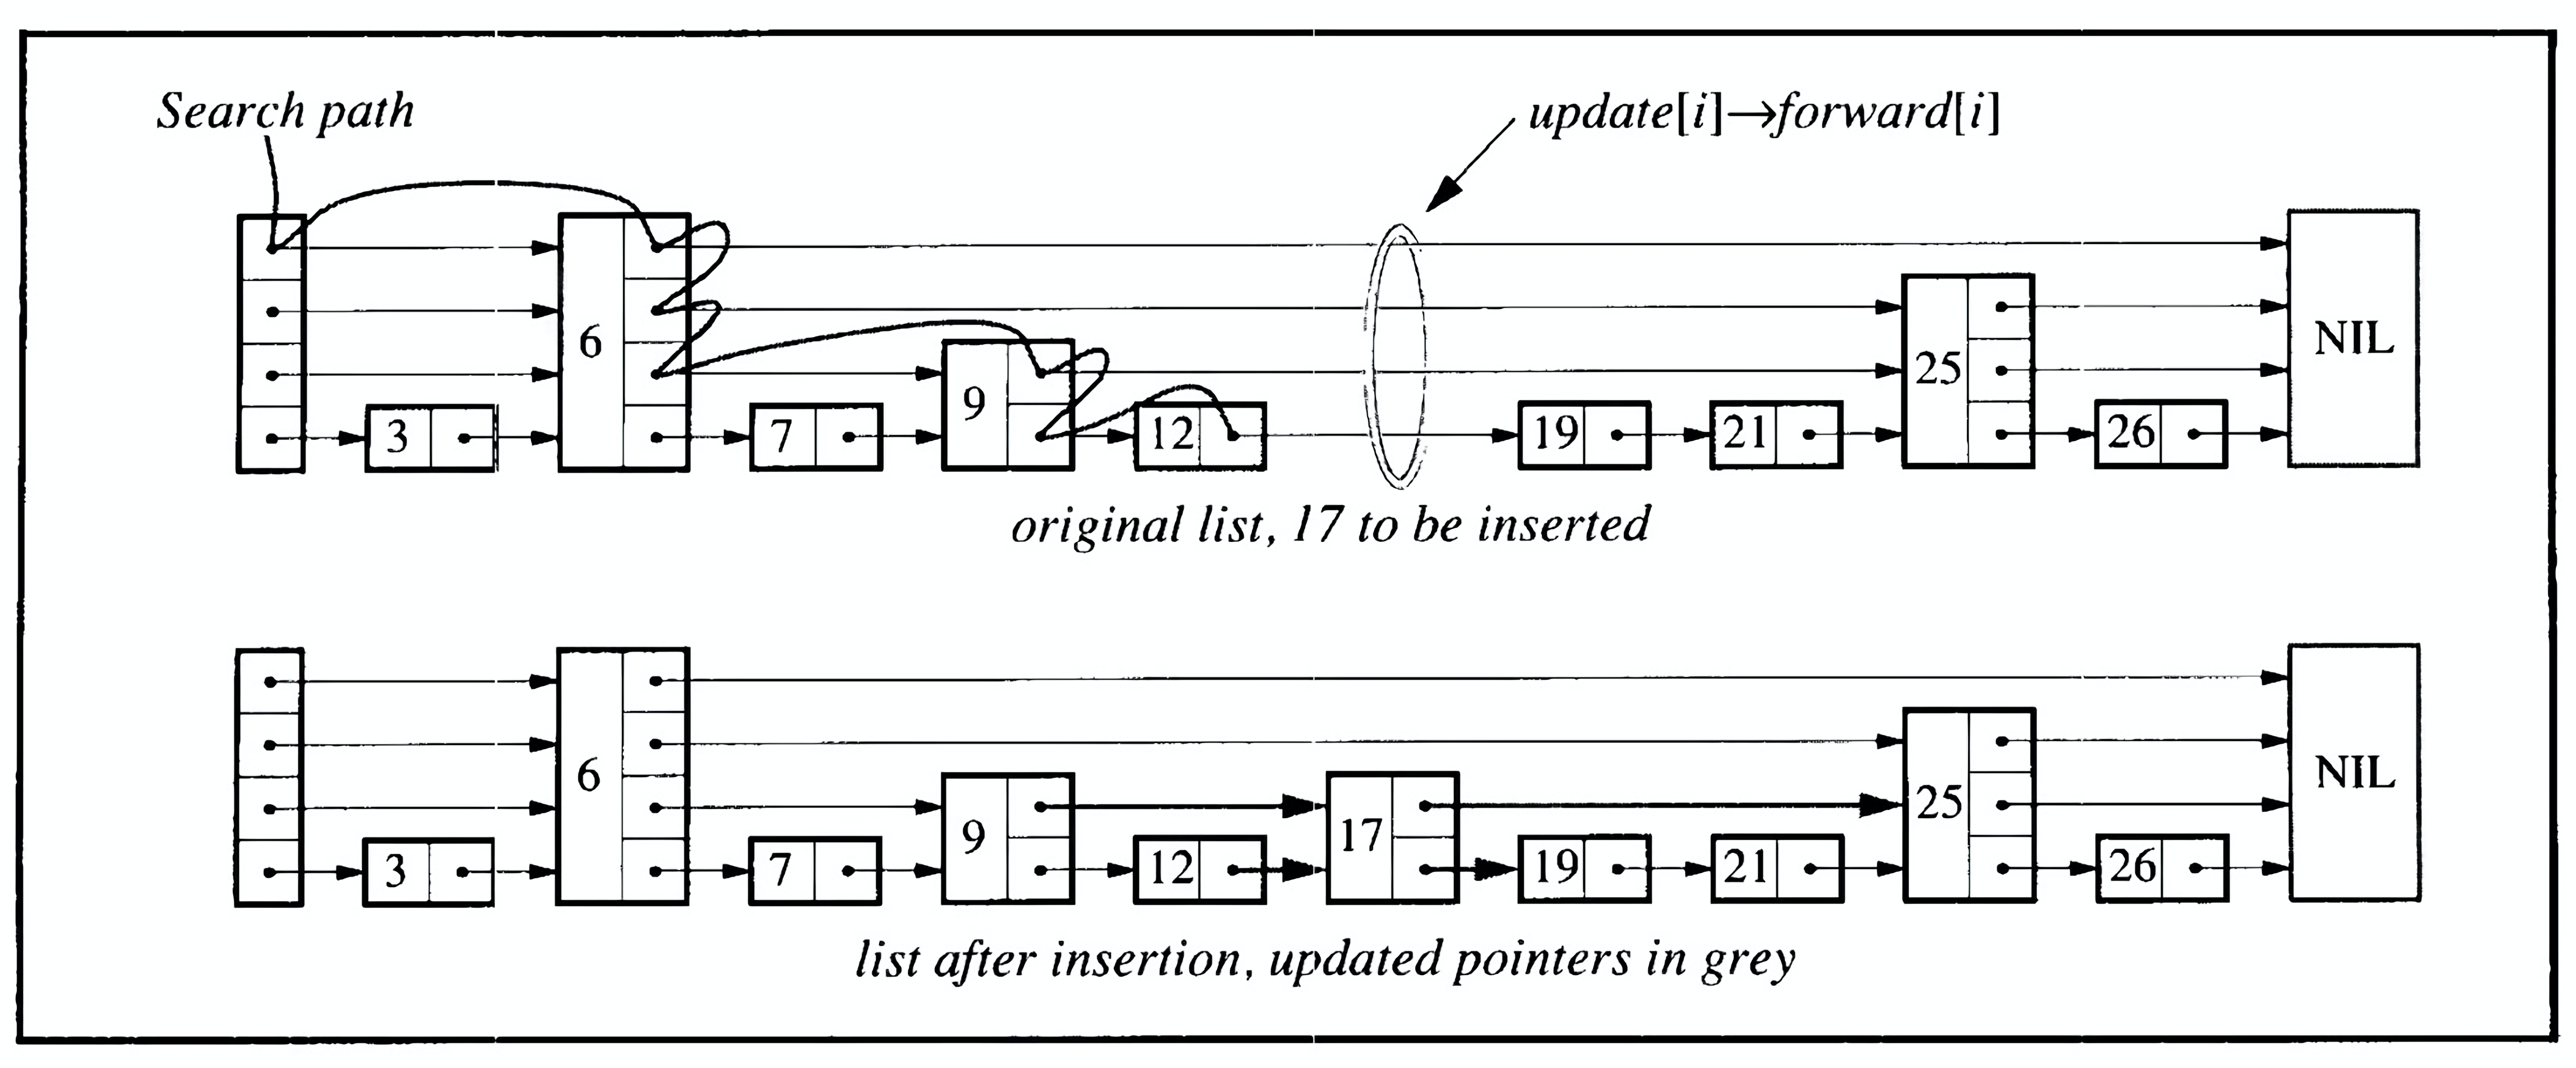
\includegraphics[scale=0.5]{Figures/Insertion}
	\caption{Pictorial Description of Steps Involved in Performing an Insertion}
\end{figure}
\begin{algorithm}[htb]
\caption{Insert(list, searchKey, newValue)}	
\begin{algorithmic}[1]
	 \Require
	 \Ensure
	 \State \textbf{local} update[1...MaxLevel]
	 \For { i:=list$\rightarrow$level \textbf{downto} 1} 
	 \While {x$\rightarrow$forward[i]$\rightarrow$key $<$ searchKey}
	 \State x:=x$\rightarrow$forward[i]
	 \State --x$\rightarrow$key $<$ searchKey $\leq$ x$\rightarrow$forward[1]$\rightarrow$key
	 \EndWhile
	 \State update[i]:=x
	 \EndFor
	 \State x:=x$\rightarrow$forward[1]
	 \If { x$\rightarrow$key = searchKey }
	 \State x$\rightarrow$value:=newValue
	 \Else
	 \State newLevel:=RandomLevel()
	 \If {newLevel $>$ list$\rightarrow$level }
	 \For {i:=list$\rightarrow$level+1 \textbf{to} newLevel}
	 \State update[i]:=list$\rightarrow$header
	 \EndFor
	 \State list$\rightarrow$level:=newLevel
	 \EndIf
	 \State x:=makeNode(newLevel, searchKey, value)
	 \For {i:=1 \textbf{to} newLevel}
	 \State x$\rightarrow$forward[i]:=update[i]$\rightarrow$forward[i]
	 \State update[i]$\rightarrow$forward[i]:=x
	 \EndFor
	 \EndIf
\end{algorithmic}
\end{algorithm}

\subsection{Delete}

\begin{algorithm}
\caption{Delete(list, searchKey, newValue)}	
\begin{algorithmic}[1]
	 \Require
	 \Ensure
	 \State \textbf{local} update[1...MaxLevel]
	 \State x:=list$\rightarrow$header
	 \For { i:=list$\rightarrow$level \textbf{downto} 1} 
	 \While {x$\rightarrow$forward[i]$\rightarrow$key $<$ searchKey}
	 \State x:=x$\rightarrow$forward[i]
	 \EndWhile
	 \State update[i]:=x
	 \EndFor
	 \State x:=x$\rightarrow$forward[1]
	 \If { x$\rightarrow$key = searchKey }
	 \For {i:=1 \textbf{to} list$\rightarrow$level}
	 \If{update[i]$\rightarrow$forward[i] $\neq$ x}
	 \State \textbf{break}
	 \EndIf
	 \State update[i]$\rightarrow$forward[i]:=x$\rightarrow$forward[i]
	 \EndFor
	 \State free(x)
	 \While {list$\rightarrow$level $>$ 1 \textbf{and} list$\rightarrow$header$\rightarrow$forward[list$\rightarrow$level] = NIL}
	 \State list$\rightarrow$level:=list$\rightarrow$level-1
	 \EndWhile
	 \EndIf
\end{algorithmic}
\end{algorithm}

\section{Main Function}



\chapter{Testing Result}
\chapter{Complexity Analysis}
The time required to excute the \texttt{Search}, \texttt{Delete} and \texttt{Insert} operation is domained by the time required to search for the appropriate element. For the \texttt{Insert} and \texttt{Delete} operations, there is an additional cost proporational to the level of the node being inserted or deleted. The time required to find an element is proportional to the length of the search path, which is determined by the pattern in which elements with different levels appears as we traverse the list.
\section{Probablistic Philosophy}
The structure of a skip list is determined only by the number of elements in the skip list and the results of consulting the random number generator. The sequence of operations that produced the current skip list does not matter. 

We assume an adversarial user does not have access to the levels of nodes; otherwise, he could create situations with worst-case running times by deleting all nodes that were not level 1. 

The probabilities of poor running times for successive operations on the same data structure are NOT independent; two successive searches for the same element will both take exactly the same time.
\section{Time Complextiy}
\subsection{Definition}
The height of the PSL is expected to be about log1/P n. Since, among all elements that made it to a certain level, about every (1/P)th element will make it to the next higher level, one should expect to make 1/p key comparisons per level. Therefore, one should expect about 1/p*log1/p n key comparisons in total, when searching for +∞. As it will turn out (Theorem 3.3), this is exactly the leading term in the search cost for $+\infty$ in a PSL of n keys.
\subsection{Search Cost}
We divide the steps on the search path into vertical steps (that is, one less than $T_n$) and horizontal steps( $L_{m-1}$ : number of full horizontal steps on the search path for the $(m-1)^{st}$ key)
\[
E\left(C_{n}^{(m)}\right)=E\left(T_{n}\right)+E\left(L_{m-1}\right)
\]

$E(T_n)$: random variables following the geometric distribution
\[
E\left(T_{n}\right)=\sum_{k \geq 1}\left\{k\left(\left(1-p^{k}\right)^{n}-\left(1-p^{k-1}\right)^{n}\right)\right\}=\sum_{k \geq 1}\left\{1-\left(1-p^{k-1}\right)^{n}\right\}
\]
$E(L_{m-1})$

\[
E\left(L_{m-1}\right)=\left\{\begin{array}{ll}
1+\frac{q}{p} \sum_{j=1}^{m-2} \sum_{k \geq 1} p^{k}\left(1-p^{k}\right)^{j} & \text { if } m=2,3, \ldots, n+1 \\
0 & \text { if } m=1
\end{array}\right.
\]
At any particular point in the climb, we are at a situation similar to situation a . We are at the ith forward pointer of a node x and we have no knowledge about the levels of nodes to the left of x or about the level of x, other than that the level of x must be at least i. Assume the x is not the header (this is equivalent to assuming the list extends infinitely to the left). If the level of x is equal to i, then we are in situation b. If the level of x is greater than i, then we are in situation c. The probability that we are in situation c is p. Each time we are in situation c, we climb up a level. We use C(k) denotes the expected cost ( length) of a search path that climbs up k levels.

An upper bound of C(k) = (L(n) - 1)/p. Because L(n) = log1/p n and p = 1/2, we can get the conclusion that C(k) = 2 * log2 n - 2 = O(log2 n)
\subsection{Insert/Delete Cost}
The Insert and Delete Algorithms are built on the Search Algorithm. After finding the position needed to insert or delete a node, the time complexity of other steps are smaller than $\mathcal O(\log n)$. So we can make a conclusion that the Insert and Delete Algorithms are both $\mathcal O(\log n)$.
\section{Space Complexity}
Every time a number is inserted, the program will randomly assign a height for node to storage pointer (less than MaxHeight), so it’s Space Complexity is $\mathcal O(n)$

\pagebreak


% Adding a bibliography if citations are used in the report
\bibliographystyle{plain}
\bibliography{bibliography.bib}
% Adds reference to the Bibliography in the ToC
\addcontentsline{toc}{chapter}{\bibname}

\pagebreak

\chapter*{Appendix A: Souce Code}
\section*{main.cpp}
\section*{SkipList.hpp}
\section*{SkipList.cpp}
\pagebreak

\chapter*{Declare}
\textit{We hereby declare that all the work done in this project titled "Skip List" is of our independent effort as a group.}
% \section{Reference solution data}


\end{document}
